\chapter{Object Detection}
L'Object Detection è un \textit{task} legato al mondo della \textit{computer vision}
che consiste nel rilevare e classificare istanze di oggetti in immagini o video.

Negli ultimi anni, grazie soprattutto all'avvento delle \ac{gpu}, c'è stato un 
incremento notevole del potere computazionale. Questo ha portato a sviluppare tecniche 
sempre più raffinate allo scopo di raggiungere prestazioni sempre migliori. 

Sempre grazie allo sviluppo di hardware sempre più potente l'interesse sta sempre 
più virando verso il mondo del \textit{Deep Learning}. 
In questo capitolo cercheremo di classificare le varie metodologie con cui si 
porta a compimento la \textit{Object Detection}. 
La letteratura sui detector è molto disomogenea e variegata, prenderemo quindi come riferimento i lavori di 
\textit{Licheng Jiao, Fan Zhang, Fang Liu, Shuyuan Yang, Lingling Li, Zhixi Feng and Rong Qu} 
\cite{DBLP:journals/corr/abs-1907-09408} e 
\textit{Zhengxia Zou, Zhenwei Shi, Yuhong Guo and Jieping Ye} \cite{DBLP:journals/corr/abs-1905-05055}.


\section{Storia della object detection}
\label{sec:history_obj}
Una prima, ma importante distinzione va fatta tra il periodo pre e post \textit{deep learning}. Il primo periodo va dagli inizi degli anni $2000$ fino al $2014$. Il secondo periodo, dove hanno preso il sopravvento tecniche basate sul \textit{deep learning}, va dal $2014$ fino ai nostri giorni. Quest'ultime tecniche possono essere a loro volta divise in altre due categorie, \textit{One Stage Detector} e \textit{Two Stage Detector} (sarà il caso di tradurre in italiano?) il cui sviluppo procede in maniera parallela. In Figura \ref{fig:history_object_detection} è presente uno schema riassuntivo con tutte le pietre miliari raggiunte durante lo sviluppo di tecniche per il rilevamento di oggetti.
\begin{figure}
    \centering
    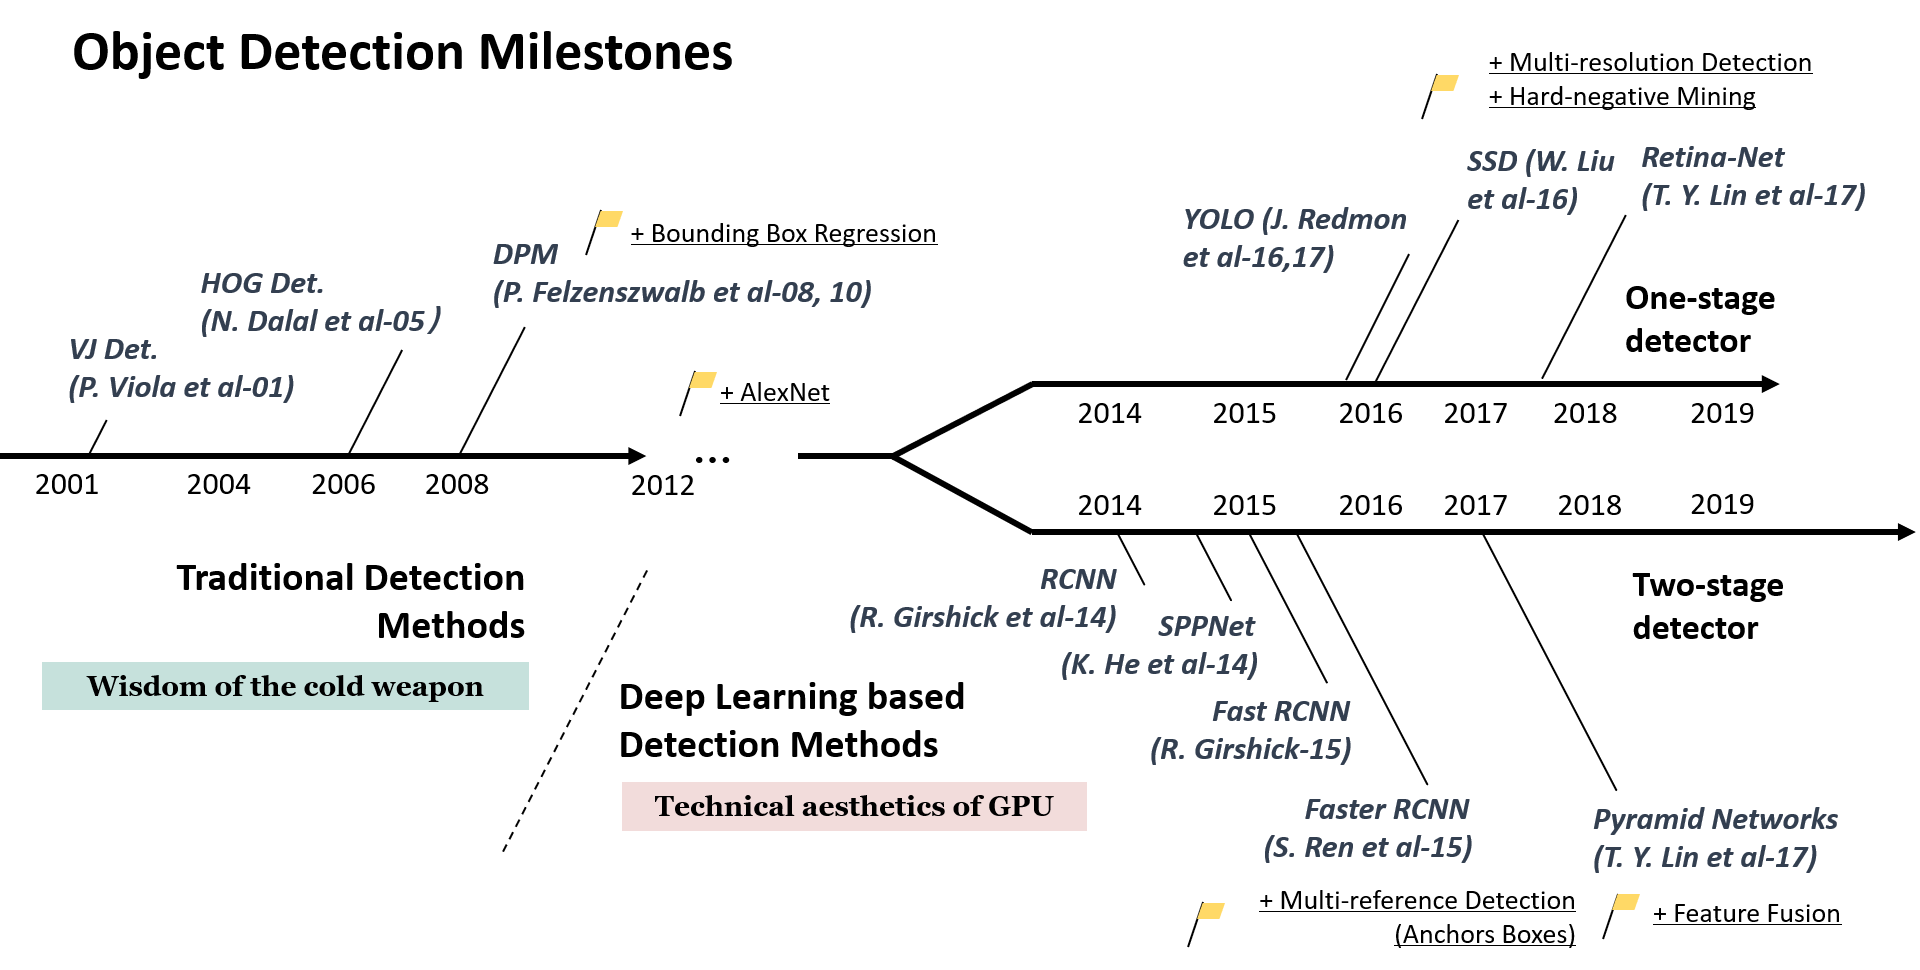
\includegraphics[width=\textwidth]{images/mile-stones.png}
    \caption{Storia della Object Detection \cite{DBLP:journals/corr/abs-1905-05055}}
    \label{fig:history_object_detection}
\end{figure}
\subsection{Evoluzione delle tecniche}
Durante questo ventennio i detector più famosi sono stati costruiti usando come mattoncini delle tecniche sviluppate ed affinate via via nel tempo. Queste tecniche sono di diverso tipo ed hanno subito evoluzioni di cui faremo una disamina nel proseguio di questa sottosezione.
\subsubsection{Prime tecniche}
Storicamente una delle prime tecniche si basava sul una teoria cognitiva chiamata \textit{Recognition by Components} \cite{biederman1987recognition}, ed è stata per molto tempo la base di alcuni lavori riguardanti il riconoscimento di immagini e la rilevazione di oggetti \cite{felzenszwalb2008discriminatively} \cite{fischler1973representation} \cite{leibe2008robust}.   

Nel passato alcuni ricercatori hanno formulato soluzioni al problema usando misure di similarità tra le componenti di un oggetto, tra la forma o i contorni, tra cui \textit{Distance Transforms} \cite{gavrila1999real}, \textit{Shape Contexts} \cite{belongie2002shape} e \textit{Edgelet} \cite{wu2005detection}.

I risultati iniziali erano molto promettenti, tuttavia quando la rilevazione è diventata più complicata queste tecniche hanno iniziato a mostrare i propri limiti, motivo per cui il passaggio al Machine Learning è stato quasi naturale. Le prime metodologie basate su questo approccio risalgono ad un periodo inquadrabile prima del $1998$, in questo caso la detection si basava su modelli statistici costruiti sopra le apparenze degli oggetti da rilevare. 
Il primo di questi modelli statistici nasce nel $1991$, chiamato \textit{Eigenfaces} \cite{turk1991eigenfaces} \cite{pentland1994view}, riesce in laboratorio a riconoscere volti in tempo reale.

Successivamente, fino al $2005$, l'evoluzione ha portato a tecniche in cui si cambiava radicalmente la rappresentazione, intesa come feature, delle immagini. Lo scopo era quindi apprendere come trasformare un immagine da insieme di pixel a insieme di coefficenti \textit{wavelet}. Grazie alla sua efficienza, tra tutte le trasformate, quella a prendere piede fu la \textit{Haar wavelet}. Dal $2005$ al $2012$ c'è stato un passaggio a rappresentazioni basate sul gradiente. 

Intorno al $1990$ iniziano a fare capolino le prime \ac{CNN} \cite{vaillant1994original} le quali però non hanno avuto grandi applicazioni per via dell'elevato costo computazionale rispetto alle risorse disponibili ai tempi. I modelli realizzati con \ac{CNN} non potevano essere quindi molto profondi, e per questo avevano forti limitazioni. Per ridurre questo elevato costo computazionale sono stati effettuati miglioramenti come \textit{space displacement network} \cite{lecun1998gradient}. Tramite questi perfezionamenti si è arrivato ad estendere ogni layer della \ac{CNN} in maniera tale da riuscire ad estrarre le feature da un immagine in un solo passaggio. Queste possono essere considerate un po' le antenate di quelle che attualmente chiamiamo \ac{FCN} \cite{long2015fully} \cite{chen2014semantic}. 
\subsubsection{Detection multiscala}
Uno degli aspetti più interessanti della ricerca si basa sulla rilevazione di oggetti con diverse misure o diverse proporzioni. Come in Figura \ref{fig:multi_scale_history} la soluzione di questo problema ha attraversato varie fasi.
\begin{figure}
    \centering
    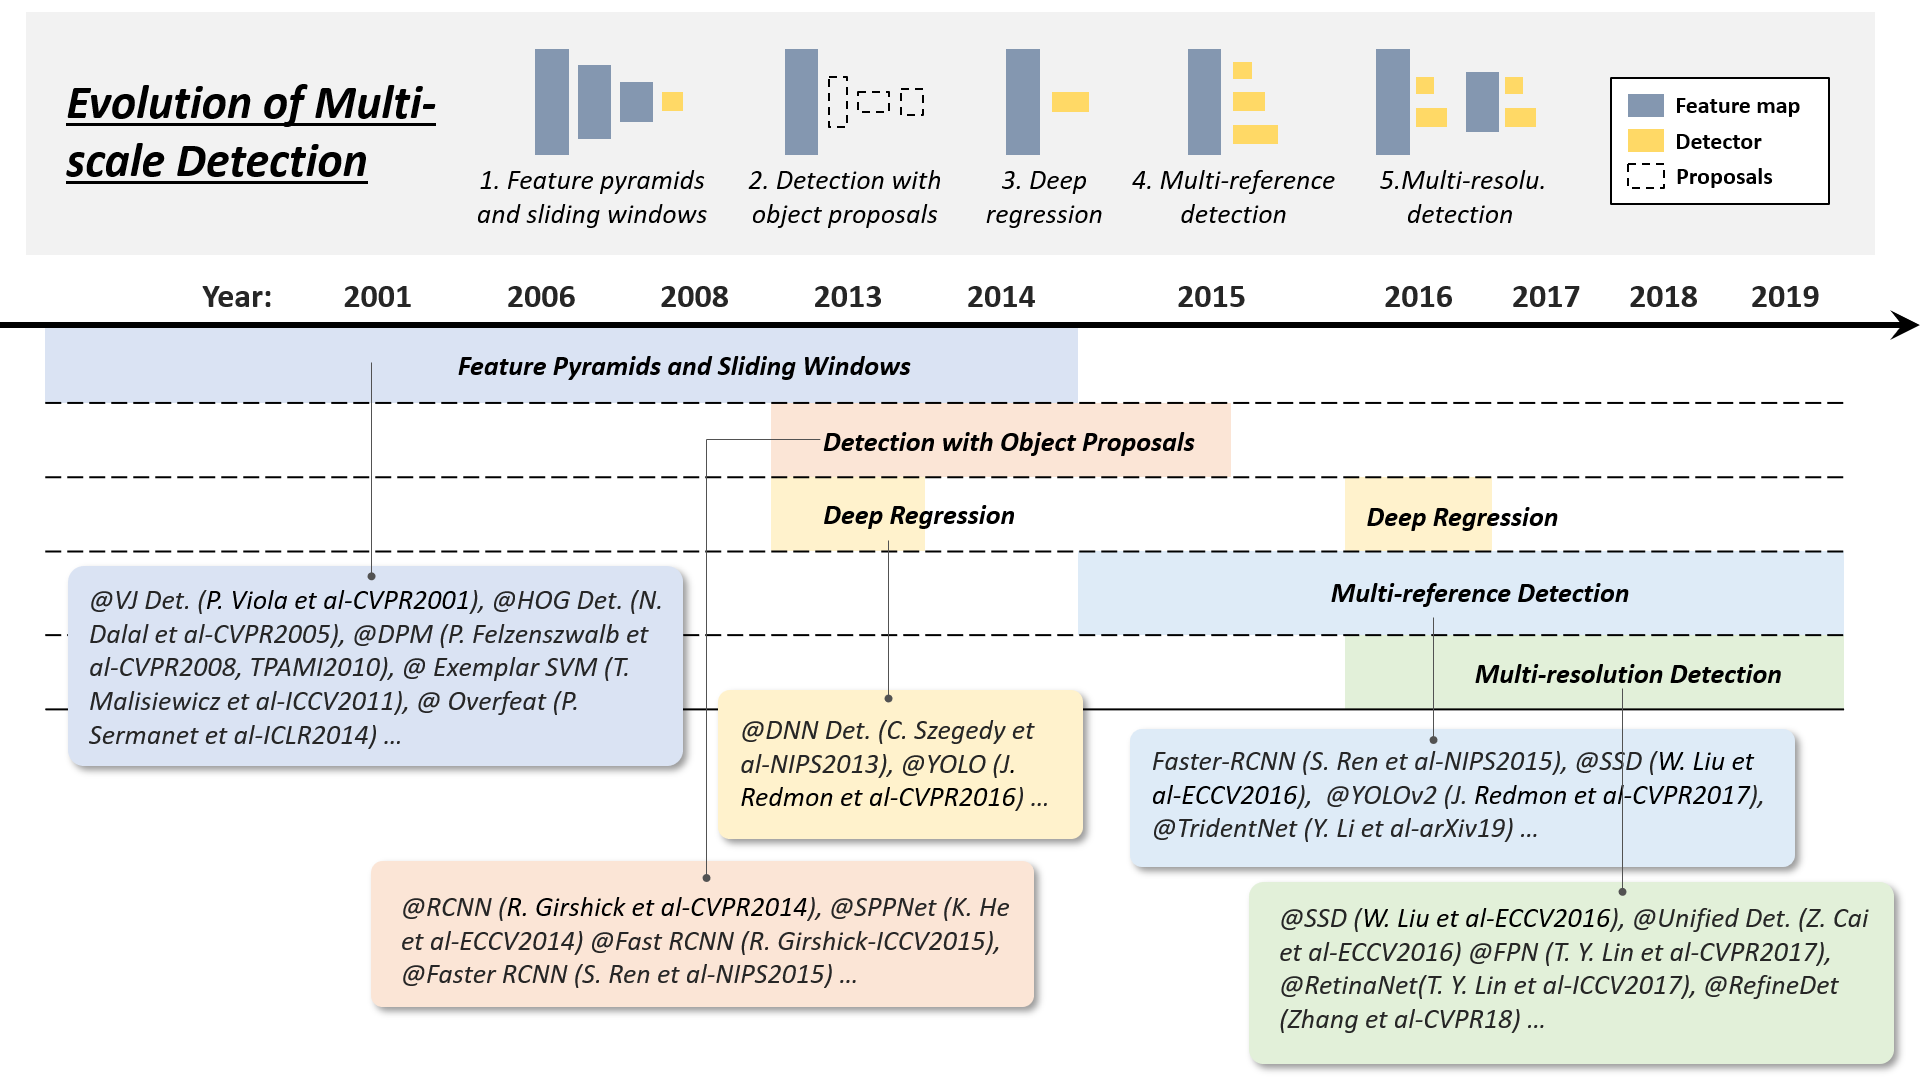
\includegraphics[width=\textwidth]{images/evol-multiscale.png}
    \caption{Evoluzione della detection multiscala \cite{DBLP:journals/corr/abs-1905-05055}}
    \label{fig:multi_scale_history}
\end{figure}
\paragraph{Feature piramidali e finestre scorrevoli}
Dal $2004$ al $2014$ sono stati creati un sacco di detector basati su questa filosofia, il problema è che erano stati disegnati con l'intento specifico di rilevare oggetti con proporzioni fisse. Ricercatori come R. Girshick \textit{et al.} iniziarono a cercare soluzioni a questo problema, arrivando a formulare un modello mistura \cite{felzenszwalb2009object} composto da più modelli addestrati su oggetti con differenti proporzioni. Sono state sviluppate anche altre soluzioni, basate questa volta sull'addestrare modelli separati per ogni istanza di oggetto dell'insieme di addestramento \cite{malisiewicz2011ensemble} \cite{malisiewicz2011exemplar}. Le limitazioni di tutte queste tecniche risidono nel fatto che i dataset più moderni sono molto diversificati, quindi l'introduzione di \textit{object proposal} ha dato ulteriore soluzione a questo problema.
\paragraph{Object Proposal}
L'idea dietro questa tecnica è creare regioni non etichettate con classi che potenzialmente possono contenere qualunque tipo di oggetto. 
Il primo avvistamento di \textit{Object Proposal} risale al $2010$ in un task di rilevazione di oggetti \cite{alexe2010object}. 
Un algoritmo di questo tipo 
\subsubsection{Regressione basata su Bounding Box}
\begin{figure}
    \centering
    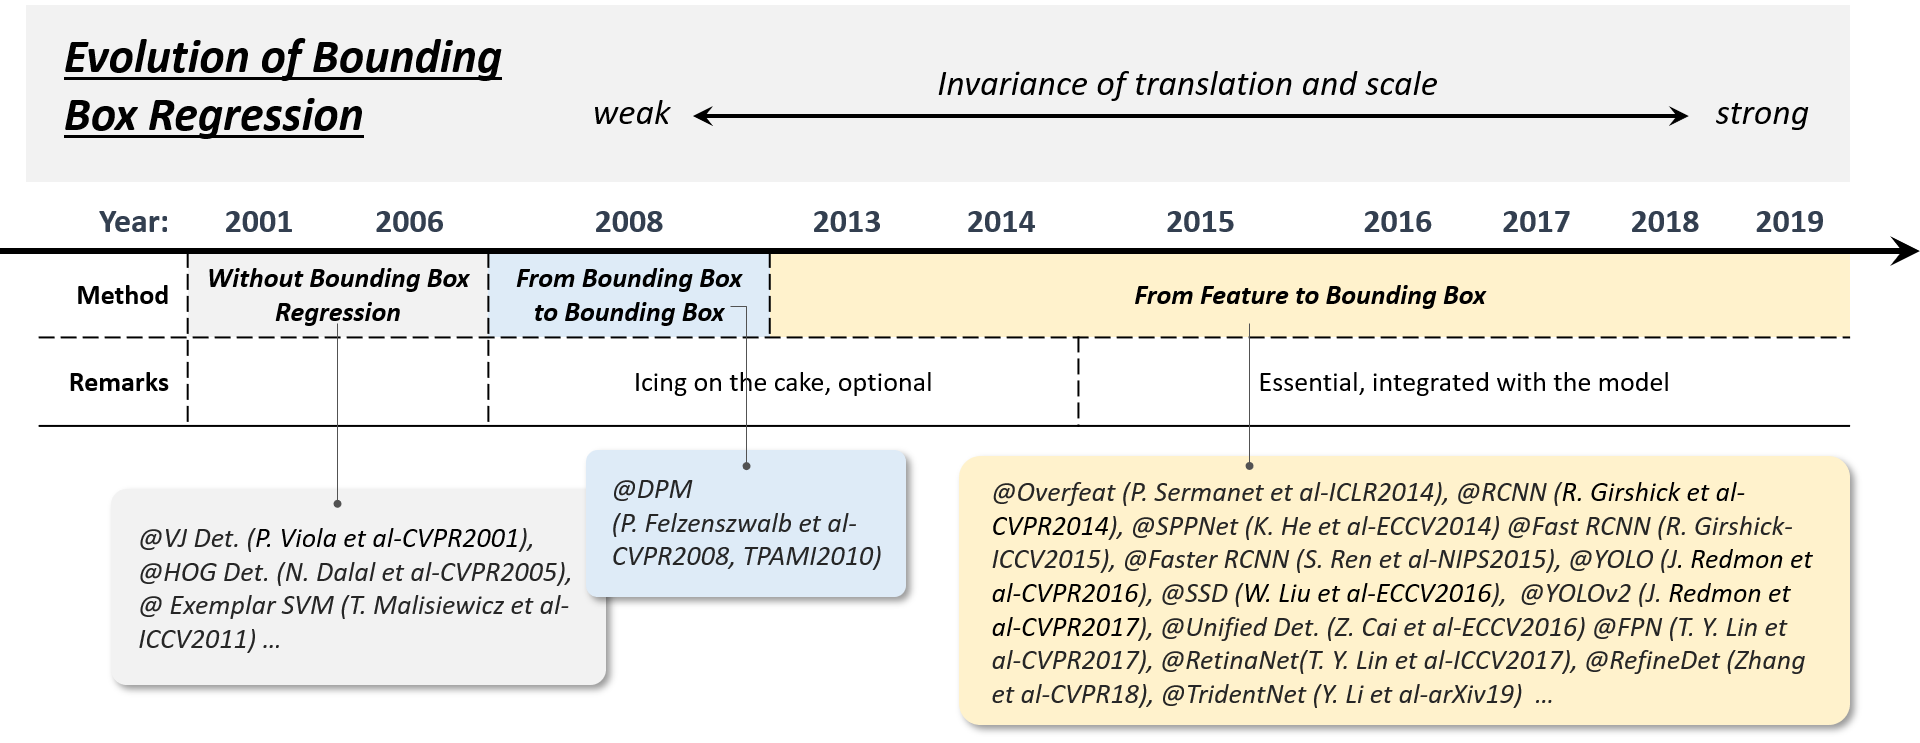
\includegraphics[width=\textwidth]{images/evol-bbreg.png}
    \caption{Evoluzione della regressione basata su \ac{BB} \cite{DBLP:journals/corr/abs-1905-05055}}
    \label{fig:bbox_history}
\end{figure}
\paragraph{Senza regressione}
\paragraph{Da BB a BB???}
\paragraph{Da feature a BB???}
\subsubsection{Context priming}
\begin{figure}
    \centering
    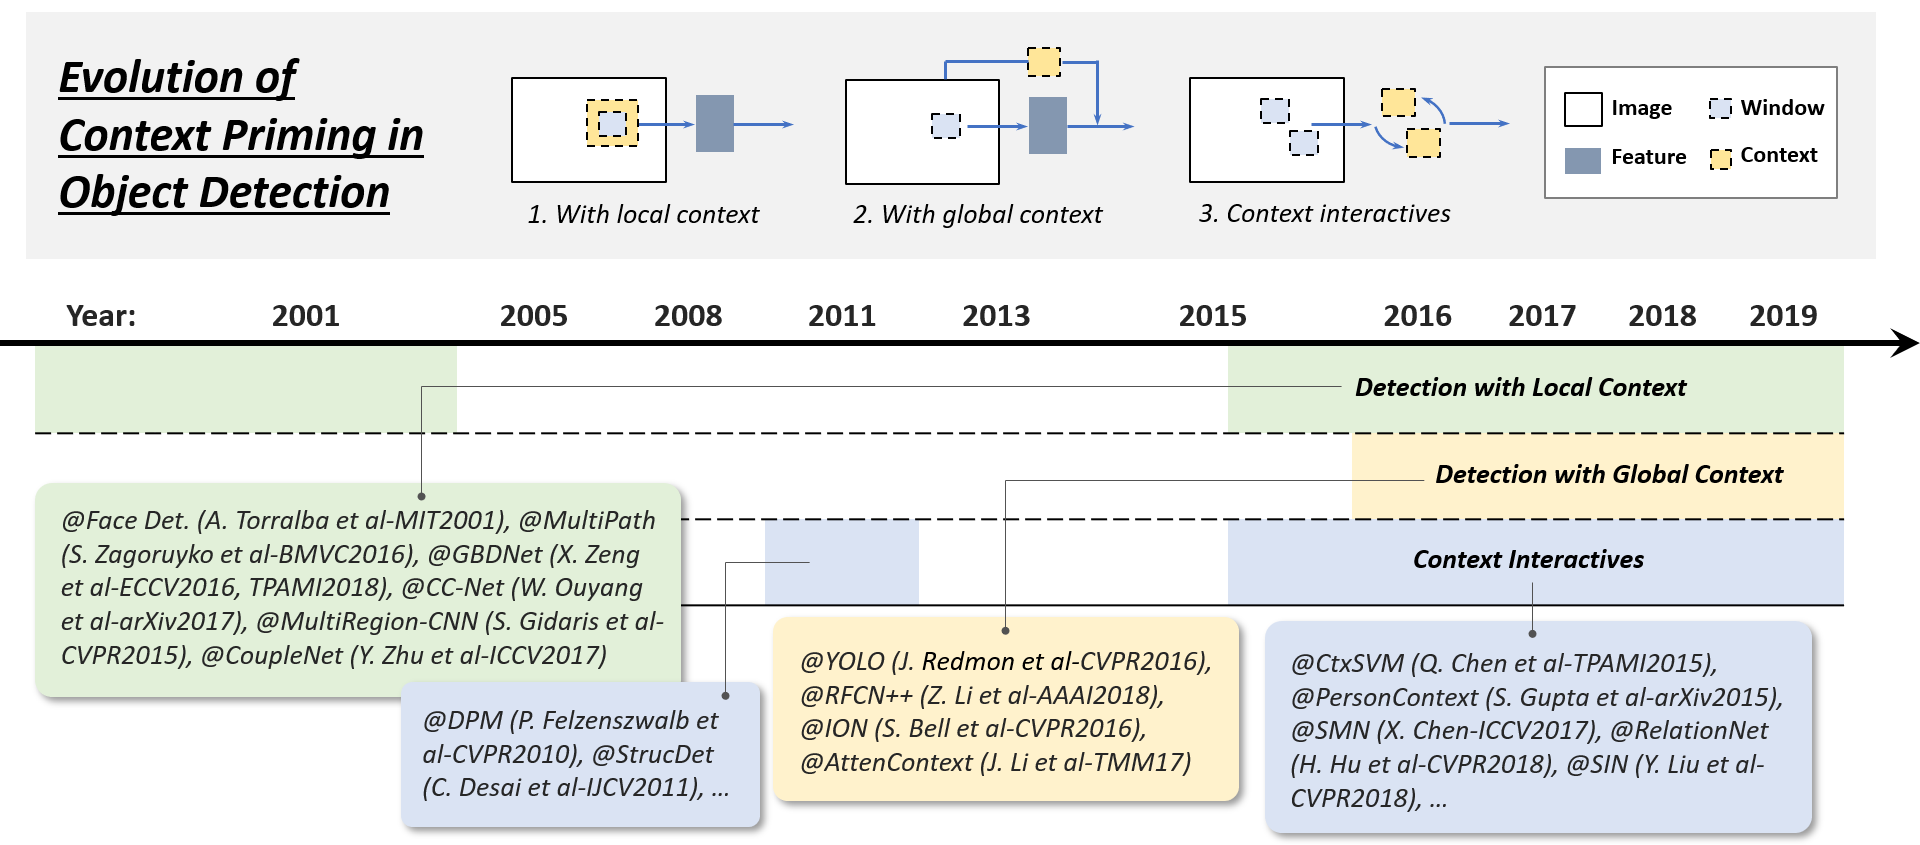
\includegraphics[width=\textwidth]{images/evol-context.png}
    \caption{Evoluzione del context priming \cite{DBLP:journals/corr/abs-1905-05055}}
    \label{fig:context_history}
\end{figure}
\paragraph{Local Context}
\paragraph{Global Context}
\paragraph{interactive context}
\subsubsection{Non Maximum Suppression}
\begin{figure}
    \centering
    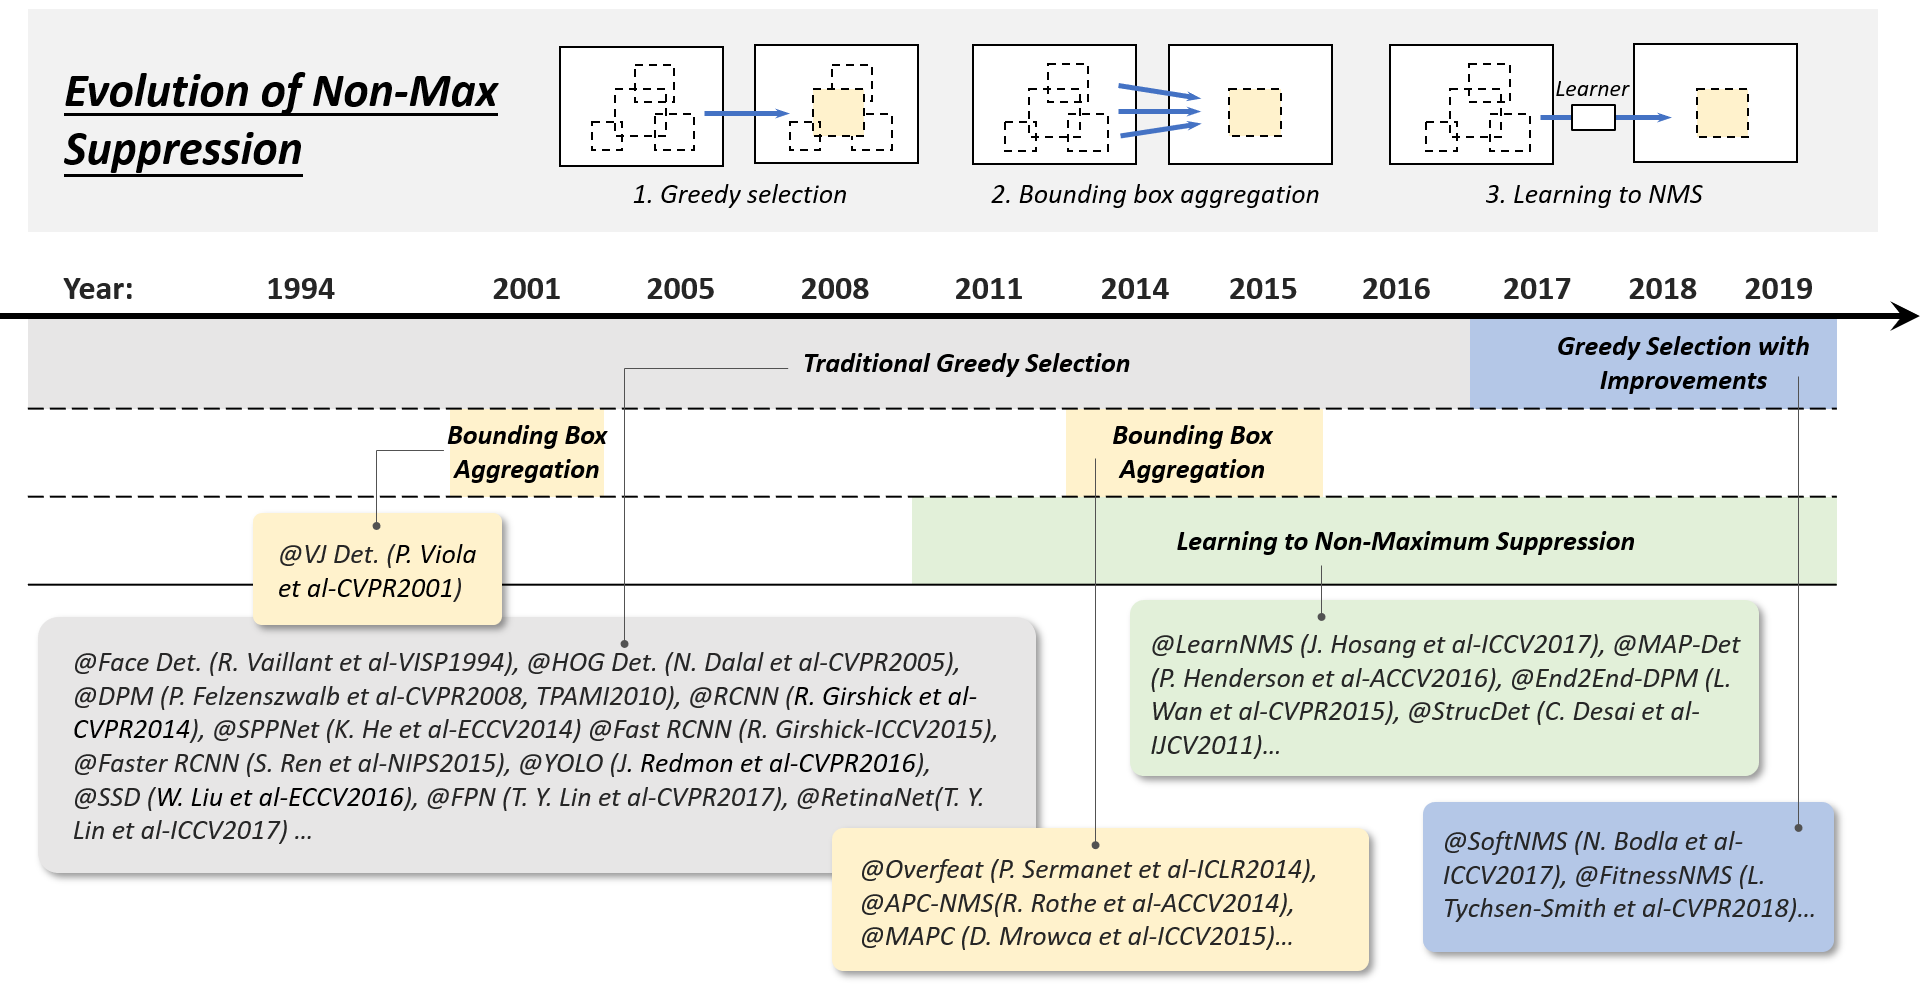
\includegraphics[width=\textwidth]{images/evol-nms.png}
    \caption{Evoluzione della Non Maximum Suppression \cite{DBLP:journals/corr/abs-1905-05055}}
    \label{fig:NMS_history}
\end{figure}
\paragraph{greedy}
\paragraph{aggregazione}
\paragraph{imparare NMS}
\subsubsection{Hard Negative Mining}
\begin{figure}
    \centering
    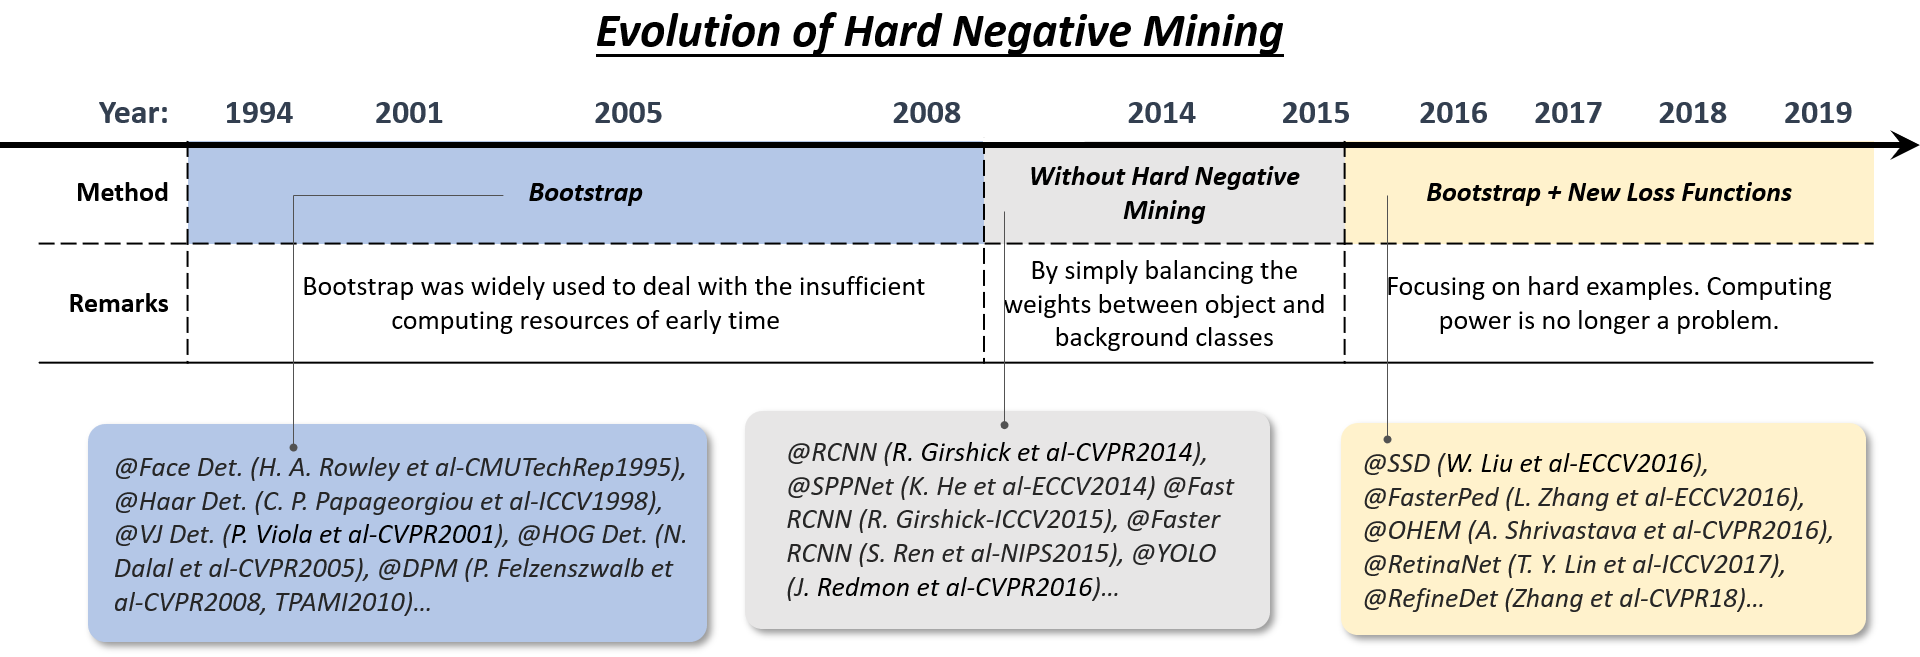
\includegraphics[width=\textwidth]{images/evol-hardnegmining.png}
    \caption{Evoluzione di Hard Negative Mining \cite{DBLP:journals/corr/abs-1905-05055}}
    \label{fig:HNM_history}
\end{figure}
\paragraph{bootstrap}
\paragraph{HNM in detector basati su deep learning}
\subsection{Dataset}
\subsection{Metriche}
\section{Detector basati su metodi tradizionali}
\label{sec:traditional_method}
\section{Detector basati su Deep learning}
\label{sec:deep_learning_obj}
\subsection{One Stage Detector}
\label{subsec:one_stage_detector}
\subsection{Two Stage Detector}
\label{subsec:two_stage_detector}

\section{RetinaNet}
\subsection{Focal Loss}